\documentclass[tikz,border=8pt]{standalone}
% Shared look for every TikZ diagram. Load with \input{../../tools/tikz-style.tex}
\usepackage[sfdefault]{roboto}
\usetikzlibrary{arrows.meta, positioning, shapes.geometric, calc, fit, backgrounds}
\definecolor{cblue}{HTML}{4C78A8}
\definecolor{corange}{HTML}{F58518}
\definecolor{cgreen}{HTML}{54A24B}
\definecolor{cred}{HTML}{E45756}
\definecolor{cpurple}{HTML}{B279A2}
\definecolor{cgrey}{HTML}{6B6B6B}
\tikzset{
  every picture/.style={font=\sffamily, line width=1.2pt},
  box/.style={draw=#1, fill=#1!12, rounded corners=4pt, align=center, inner sep=7pt, minimum height=1.1cm},
  box/.default=cgrey,
  arrow/.style={-{Stealth[length=3mm]}, draw=cgrey, line width=1.4pt},
  title/.style={font=\sffamily\bfseries\Large},
  note/.style={font=\sffamily\small, text=cgrey, align=center},
}
\AtBeginDocument{\hyphenpenalty=10000 \exhyphenpenalty=10000}

% The consistency (triangle) rule h(n) <= c(n, n') + h(n'), checked on one move of each example.
% Left: the grid, cell n = x 2.5-3.0, y 2.5-3.0 m to the cell above it, n'; octile guesses 1.414 and 1.207 m
% (searchkit.octile), move 0.500 m: 1.414 <= 1.707, holds. Right: the roadmap, A to C, 0.906 m; h(A) = 2.072 m
% (remembered), h(C) = 0: 2.072 > 0.906, fails (counterexample.py).
\begin{document}
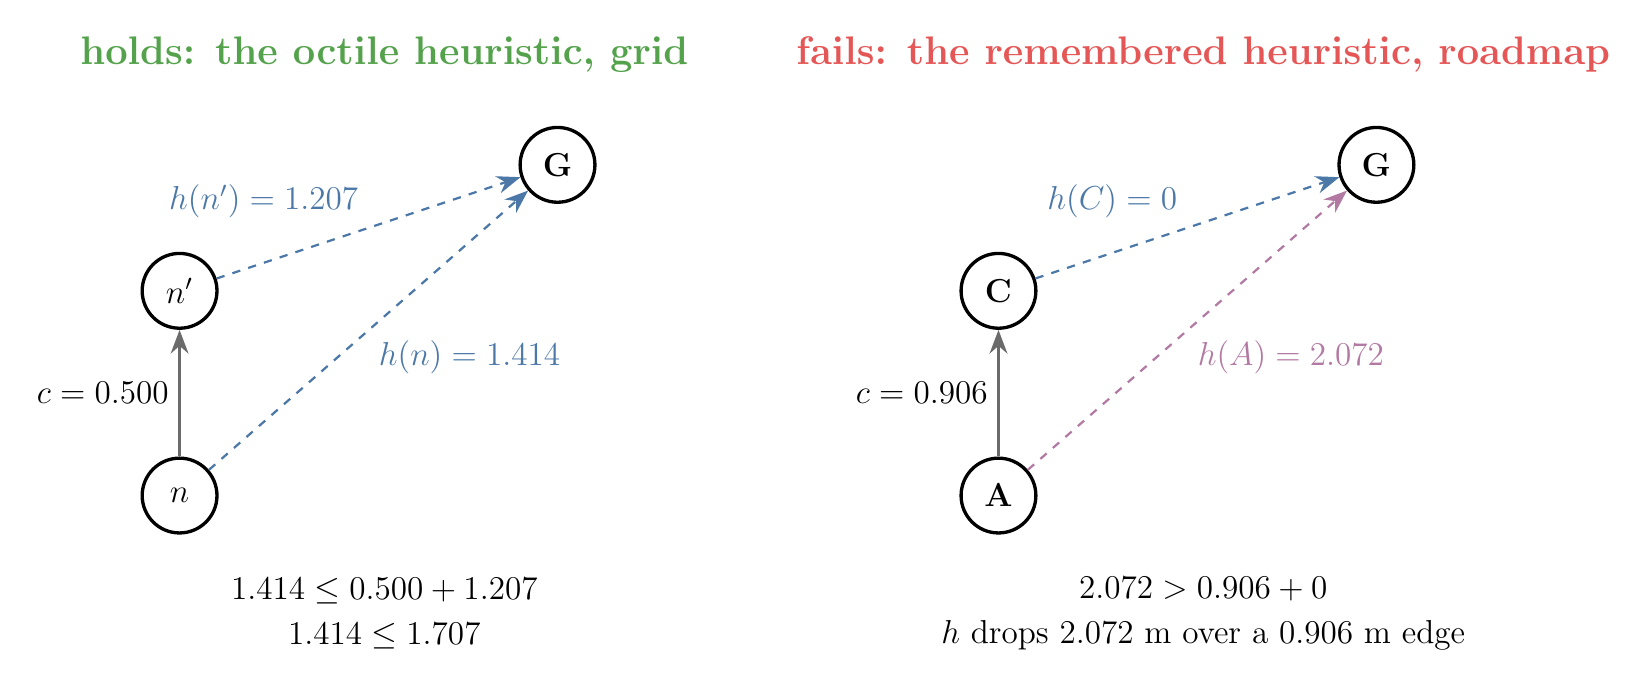
\begin{tikzpicture}[every node/.append style={font=\large},
  pt/.style={circle, draw=black, fill=white, minimum size=0.95cm, inner sep=0pt, font=\large\bfseries}]
  % left: holds
  \node[font=\Large\bfseries, text=cgreen] at (2.6,5.6) {holds: the octile heuristic, grid};
  \node[pt] (n) at (0,0) {$n$};
  \node[pt] (m) at (0,2.6) {$n'$};
  \node[pt] (g) at (4.8,4.2) {G};
  \draw[arrow, very thick] (n) -- node[left] {$c = 0.500$} (m);
  \draw[arrow, dashed, cblue, thick] (n) -- node[below right, text=cblue] {$h(n) = 1.414$} (g);
  \draw[arrow, dashed, cblue, thick] (m) -- node[above left, text=cblue] {$h(n') = 1.207$} (g);
  \node[align=center] at (2.6,-1.5) {$1.414 \le 0.500 + 1.207$\\[2pt] $1.414 \le 1.707$};
  % right: fails
  \begin{scope}[xshift=10.4cm]
  \node[font=\Large\bfseries, text=cred] at (2.6,5.6) {fails: the remembered heuristic, roadmap};
  \node[pt] (a) at (0,0) {A};
  \node[pt] (c) at (0,2.6) {C};
  \node[pt] (g2) at (4.8,4.2) {G};
  \draw[arrow, very thick] (a) -- node[left] {$c = 0.906$} (c);
  \draw[arrow, dashed, cpurple, thick] (a) -- node[below right, text=cpurple] {$h(A) = 2.072$} (g2);
  \draw[arrow, dashed, cblue, thick] (c) -- node[above left, text=cblue] {$h(C) = 0$} (g2);
  \node[align=center] at (2.6,-1.5) {$2.072 > 0.906 + 0$\\[2pt] $h$ drops 2.072 m over a 0.906 m edge};
  \end{scope}
\end{tikzpicture}
\end{document}
